% Diese Zeile bitte -nicht- aendern.
\documentclass[course=erap]{aspdoc}
\usepackage{wrapfig}
\usepackage{graphicx}
\usepackage{blindtext}
\usepackage{listings}

%%%%%%%%%%%%%%%%%%%%%%%%%%%%%%%%%
%% TODO: Ersetzen Sie in den folgenden Zeilen die entsprechenden -Texte-
%% mit den richtigen Werten.
\newcommand{\theGroup}{188} % Beispiel: 42
\newcommand{\theNumber}{A325} % Beispiel: A123
\author{Lukas Michael Englhauser \and Thua Duc Nguyen \and Michal Klakus}
\date{Sommersemester 2022} % Beispiel: Wintersemester 2019/20
%%%%%%%%%%%%%%%%%%%%%%%%%%%%%%%%%
% Diese Zeile bitte -nicht- aendern.
\title{Gruppe \theGroup{} -- Abgabe zu Aufgabe \theNumber}

\begin{document}
	\maketitle
	
	\section{Einleitung}
	
	Die Quadratwurzel von 2 ist eine positive reelle Zahl, 
	die mit sich selbst multipliziert die Zahl 2 ergibt. In der Mathematik 
	kann sie geschrieben werden als \(\sqrt{2}\) und ist eine 
	algebraische Zahl. Sie war die erste reelle Zahl, die als irrational entdeckt wurde.
	\newline
	Geometrisch gesehen ist die Quadratwurzel aus 2 die Länge einer Diagonale durch ein 
	Quadrat mit Seiten von einer Einheit Länge. Dies ergibt sich aus dem Satz des Pythagoras.
	\newline
	\begin{figure}[h]
		\centering
		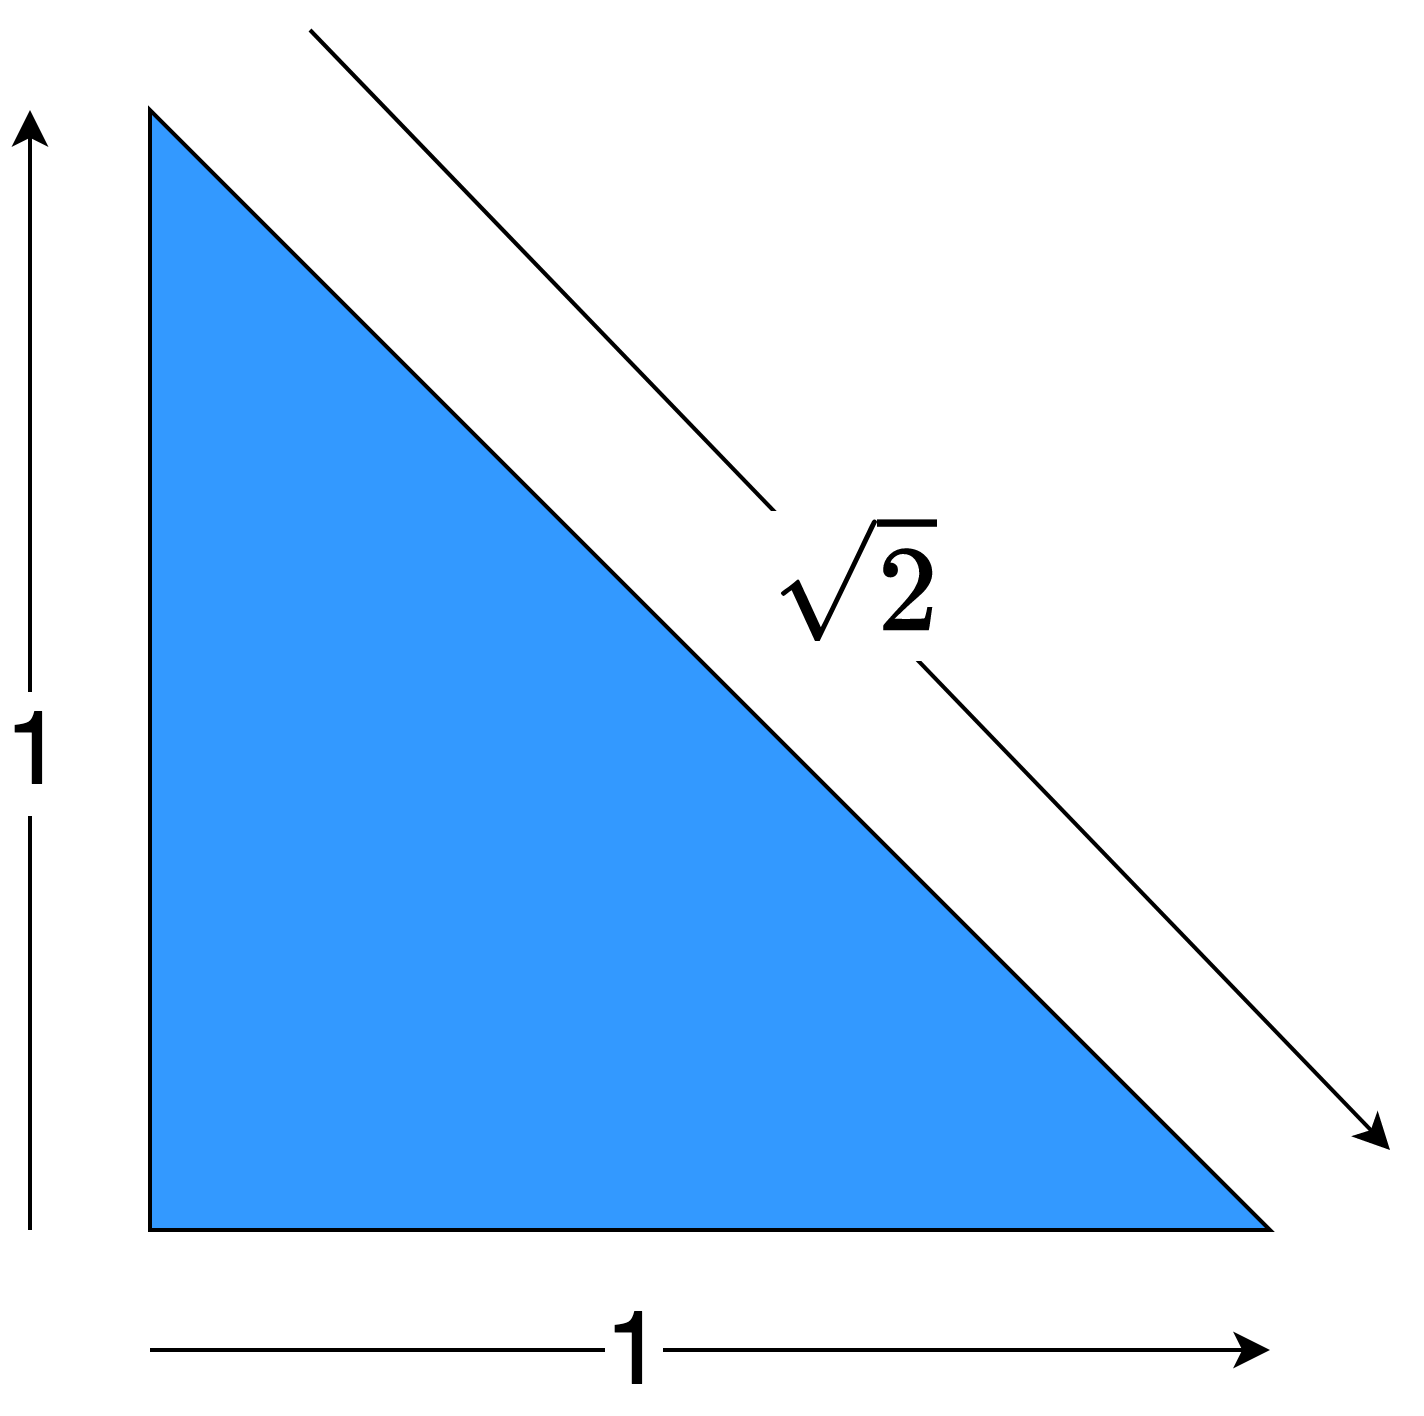
\includegraphics[width=0.2\textwidth]{Abbildungen/triangle.png}
		\caption{Bedeutung von $\sqrt{2}$ in der realen Welt}
	\end{figure}
	\newline
	Da $\sqrt{2}$, wie alle reellen Zahlen, unendlich viele Nachkommastellen hat, kann sie nicht genau berechnet, sondern nur mit der folgenden mathematischen Gleichung angenähert werden:
	\begin{equation*}
		\sqrt{2} = 1 + \sum_{i=1}^{\infty} \prod_{k=1}^{i} \frac{2k-1}{4k}
	\end{equation*}
	In diesem Projekt ist diese effizient zu implementieren, um die Konstante mit beliebiger, konfigurierbarer Genauigkeit zu berechnen und in einem Rahmenprogramm mit verschiedenen Optionen zugänglich zu machen. Für die effiziente Berechnung des obigen Terms ist die Verwendung des Binary Splitting und für die Multiplikation zweier Zahlen die der Karazuba-Multiplikation in der Aufgabenstellung vorgeschrieben. Für alle anderen Rechenoperationen ist selbst eine Lösung zu finden.
	Wir werden unseren Ansatz präsentieren, und die Qualität
	unserer Lösung wissenschaftlich bewerten.\newpage
	
	\section{Lösungsansatz}
	
	\subsection{Darstellung großer Zahlen}
	\subsubsection{Bignum}
	Die Berechnung von beliebiger Anzahl der Nachkommastellen von \(\sqrt{2}\) lässt sich nicht mithilfe von den standardmäßigen Datentypen realisieren.\newline
	
	Hierfür wird eine Datenstruktur namens bignum eingeführt, die eine Zahl in einem Feld von 32 Bit unsigned Integern abspeichert. Für diese Zellen Größe haben wir uns entschieden, da so die Multiplikation zweier Zellen im Gegensatz zu 64 Bit Größe ohne das Problem des Erhaltens der höherstelligen Bits möglich ist. Ein Nachteil ist so aber, dass insgesamt mehr Multiplikationen Durchgeführt werden müssen.
	
	Die Zahl die von bignum repräsentiert wird entspricht dem dezimalen Äquivalent der Aneinanderreihung der einzelnen Blöcke in der richtigen Reihenfolge. Zusätzlich werden noch die Anzahl der belegten Blöcke und Nachkommablöcke gespeichert. \newline
	
	\begin{lstlisting}
		struct bignum {
			uint32_t *numbers;
			size_t length;
			size_t subone;
		};
	\end{lstlisting}
	Es ist erwähnenswert, dass man bei den meisten arithmetischen Operationen der Multi-Byte Zahlen, die Berechnungen mit dem niederwertigsten Block beginnen muss. Anderenfalls kann es zu falschen Ergebnissen kommen, beispielsweise wegen der unbeachteter Carry-Flag. Aus diesem Grund wird das Little-Endian Format genutzt. In der nullten Zelle des Feldes steht also der Block mit der geringsten Wertigkeit.
	
	\subsubsection{Darstellung von Nachkommastellen} 
	Die Nachkommastellen werden immer in ganzen Blöcken dargestellt. Dieses Format wurde gewählt, weil es einige Operationen vereinfacht.
	Zum Beispiel ist es so nach einer Addition leichter zu ermitteln, wo die Nachkommastellen der Summe beginnen.\newline
	
	
	Die Verwendung von Fließkommazahlen nach IEEE-754 ist nicht geeignet, da auch das Rechnen mit großen Ganzzahlen möglich sein muss und diese Art der Zahlendarstellung in diesem Fall zu sehr an Genauigkeit verliert.
	Ansonsten müsste die Mantisse die gleiche Anzahl an Bits wie eine reguläre Darstellung der Zahl beinhalten, was die Sinnhaftigkeit der Verwendung von Fließkommazahlen untergraben würde.\newline
	
	
	Um unnötigen Rechenaufwand und Speicherbelegung zu verhindern wird in unserer Implementierung auf die Darstellung von Nachkommastellen, die den Wert der Zahl nicht beeinflussen, also am Ende der Zahl stehen und Null sind, verzichtet.
	Eine weitere Möglichkeit der Darstellung ist eine Variable, die die Anzahl der Dezimal-Bits angibt. Da die Arithmetik aber ohnehin immer Blockweise ablaufen muss haben wir uns nicht für diese Variante entschieden.
	
	\subsection{Arithmetik}
	Um mithilfe von einer solcher Datenstruktur arbeiten zu können, wird sowohl Ganzzahlarithmetik als auch die Rechnung mit Nachkommastellen benötigt. Während die Methoden zur Subtraktion und Addition relativ unkompliziert ist, benötigt man für die Multiplikation und Division besondere Verfahren, insbesondere wenn die Operationen gute Performanz haben sollen.
	Wie von der Aufgabenstellung verlangt verwenden wir für das Bestimmen von Produkten die Karazuba-Multiplikation. Für das Ermitteln von Quotienten haben wir die Newton-Raphson-Division herangezogen.
	
	\subsubsection{Addition/Subtraktion}
	Es ist bei der Berechnung der Addition bzw. Subtraktion zweier Zahlen erforderlich darauf zu achten, dass nur Zahlen gleicher Wertigkeit verrechnet werden. Bei der Addition kann im Fall, dass eine Zahl genauer ist, kann deren Wert an diesen Blöcken einfach übertragen werden.
	
	Bei der Subtraktion kommt es zu einer Subtraktion von Null, die zu einem Underflow führt. Dieses Verhalten ist prinzipiell erwünscht, da es mit der Subtraktion eines Übertragsbits von einem höherwertigen Block zum richtigen Ergebnis führt.
	Da Subtraktionen, in denen der Subtrahend größer als der Minuend ist für diese Aufgabe keine Rolle spielen, ist deren Ergebnis in unserer Implementierung nicht eindeutig definiert.
	
	Da bei einer Gleichzeitigen Addition bzw. Subtraktion von aufeinanderfolgenden Werten Überträge entstehen können, die im jeweils nächst höheren Wert wieder zu Überträgen führen können und so wieder mehrmaliges Addieren und ein Verfahren zur Erkennung von Überträgen notwendig ist, haben wir uns gegen die Nutzung von SIMD entschieden.
	
	\subsubsection{Karazuba-Multiplikation}
	Trotz der Tatsache, dass moderne Prozessoren zwei standardmäßige Zahlen miteinander schnell und effektiv multiplizieren können, ist eine effiziente Berechnung von größeren Eingaben herausfordernder. Da in diesem Programm in der Regel mit der obig beschrieben Struktur gearbeitet wird, muss die Multiplikation dafür adaptiert werden.\newline
	Eine naive Implementierung von dieser Operation besteht darin, dem \glqq Schulprozess\grqq zu folgen. Der Algorithmus gehört aber zu einer Laufzeitklasse von $\Theta(n^2)$, weshalb er für unsere Zwecke absolut ungeeignet ist.
	
	Eine möglich Verbesserung kann der Karazuba-Multiplikation Algorithmus bereitstellen. Dieser sieht wie folgt aus:
	
	1. Die zu multiplizierenden Zahlen $x$,$y$ werden auf zwei Teile, jeweils von $p$ Bits geteilt, sodass
	
	\begin{equation*}
		\centering
		x = x_0 + x_1*2^{\frac{m}{2}}
	\end{equation*}
	
	
	\begin{equation*}
		\centering
		y = y_0 + y_1*2^{\frac{m}{2}}
	\end{equation*}
	
	Laut Karazuba-Multiplikations Verfahren lässt sich die Multiplikation von x und y mittels oben genannten Summen folglich darstellen:
	
	\begin{equation*}
		x\cdot y= x_0y_0 + 2^p((x_0+y_0)(x_1+y_1) - x_0y_1 - x_1y_1) + 2^{2m}x_1y_1    
		\cite{Karatsuba} 	
	\end{equation*}
	
	Der Algorithmus wird rekursiv aufgerufen, bis man bei zwei Zahlen angekommen ist, die sich effizient miteinander multiplizieren lassen.
	Dies ermöglicht die Anzahl von Multiplikationen der Zahlen $x = x_0 + x_1*2^{\frac{m}{2}}$ und $y = y_0 + y_1*2^{\frac{m}{2}}$ von vier auf drei zu verringern.  Damit verbessert sich theoretisch die Laufzeit der Implementierung von $\theta(n^2)$ zu 
	$O(n^{log 3}) \approx O(n^{1.59})$. \newline
	
	Um zwei große Zahlen auf diese Art und Weise multiplizieren zu können, müssen sie aber drei Voraussetzungen erfüllen. 
	\begin{itemize}
		\item Beide Zahlen müssen die gleiche Anzahl von Bits haben. 
		\item Die Hälfte der Anzahl der Bits beider Zahlen muss ein Vielfaches der minimalen Berechnungsgröße, hier also 32 Bit, sein.
		\item Die Anzahl der Nachkommastellen muss identisch sein.
	\end{itemize}
	
	Zwei Zahlen können zu diesen Eigenschaften konform gemacht werden: Die Zahl mit weniger Nachkommablöcken wird um die Differenz zur Anzahl der anderen mit Null-Blöcken an der Position mit geringster Wertigkeit erweitert. Dann muss man die Zahlen an den höchstwertigen Stellen mit Null-Blöcken erweitern, bis bei beiden die gleiche, gerade Anzahl von Blöcken erreicht ist.\newline
	
	Für das Rechnen mit Werten die keine Ganzzahlen sind werden die Zahlen wie oben beschrieben konform gemacht und dann so, als wären sie Ganzzahlen miteinander verrechnet. Die Anzahl der Nachkommablöcke des Produkts entspricht dann der Summe derer der beiden konformen Zahlen, bzw. dem Doppelten der Nachkommablöcke der genaueren Zahl.\newline 
	
	Auch hier ist SIMD wieder nicht sinnvoll, da die einzelnen Rekursionsschritte nicht verringert werden kann und somit ein geringer Leistungsgewinn zu erwarten ist.
	
	\subsubsection{Newton–Raphson Verfahren}
	Die Division mit dem Newton-Raphson Verfahren berechnet einen Quotienten, indem eine Annäherung des Kehrwertes des Nenners ermittelt und anschließend mit dem Zähler multipliziert wird. Dabei werden nur die Operationen der Multiplikation und Subtraktion benötigt. Es wird von einer anfänglichen Abschätzung ausgehend iterativ ein immer genaueres Ergebnis berechnet. 
	
	Um diese berechnen zu können wird der Nenner auf einen Wert zwischen $0,5$ und $1$ \glqq normalisiert\grqq. Dies erfolgt durch Bitshifts nach rechts, bis das erste Nachkommabit Eins ist. Um dennoch noch auf ein korrektes Ergebnis zu kommen muss dieselbe Anzahl an Rechtsverschiebungen auch auf den Zähler angewendet werden.\newline 
	
	Die Formel für die nächste Annäherung an den Kehrwert des normalisierten Nenners $N$ ist dabei:
	\begin{equation*}
		x\textsubscript{n +1} = x\textsubscript{n}(2 - N*x\textsubscript{n})
	\end{equation*}
	
	Die Division und somit auch die Rechtsverschiebungen der Nenners und Zählers werden für jede Eingabe genau einmal ausgeführt. Pro Iteration werden zwei Multiplikationen und eine Subtraktion benötigt, weshalb Optimierungen vor allem in den grundlegenderen Operationen sinnvoll ist.\newline
	
	Da die Berechnung der Annäherung des Kehrwerts und anschließend die Multiplikation mit dem Zähler sequentiell aufeinander aufbauen und die Zahlen ohnehin zu groß für einzelne Register sind, ist der Einsatz von SIMD auch hier nicht möglich.\newline
	
	Ein anderes mögliches Verfahren ist die Goldschmidt-Division. Diese braucht pro Iteration zwei unabhängige Multiplikationen und ist deshalb mit Parallelisierung schneller als Newton-Raphson. Da das benutzen mehrerer Threads aber nicht Teil des Praktikums ist, haben wir uns gegen deren Einsatz entschieden.
	
	\subsection{Binary Splitting}
	Die gegebene Gleichung 
	\begin{equation}
		\sqrt{2} = 1 + \sum_{i=1}^{\infty} \prod_{k=1}^{i} \frac{1 \times (2k-1)}{1 \times 4k}
	\end{equation} 
	ist eine linear konvergente Reihe und sie kann effizient mittels Binary Splitting berechnet werden. Sei $S_{n_1, n_2}$ für $n_1, n_2 \in N$ mit $n_1 < n_2$ eine Folge der folgenden Form und seien $a(n) = 1, b(n) = 1, p(n) = 2n - 1, q(n) = 4n$ Polynome in n mit ganzzahligen Koeffizienten, können wir (1) umformulieren: 
	\begin{equation*}
		\sqrt{2} = \frac{a(n)}{b(n)} \times \frac{p(n_1) . . . p(n)}{q(n_1) . . . q(n)}
	\end{equation*} 
	Zur Berechnung werden folgende Hilfsterme mit $n_m = \lfloor n_1 + n_2 \rfloor$ rekursiv definiert:
	\begin{equation*}
		P_{n_1,n_2} = p(n_1) ... p(n_2 - 1) =  \left\{ \begin{array}{rcl}		
			p(n_1)  & \mbox{if} & n_1 = n_2 - 1  \\
			P_{n_1,n_m},P_{n_m,n_2}  & \mbox{ } &  otherwise			
		\end{array}\right.
	\end{equation*}
	
	\begin{equation*}
		Q_{n_1,n_2} = q(n_1) ... q(n_2 - 1) =  \left\{ \begin{array}{rcl}		
			q(n_1)  & \mbox{if} & n_1 = n_2 - 1  \\
			Q_{n_1,n_m},Q_{n_m,n_2}  & \mbox{ } &  otherwise			
		\end{array}\right.
	\end{equation*}	
	
	\begin{equation*}
		B_{n_1,n_2} = b(n_1) ... b(n_2 - 1) =  \left\{ \begin{array}{rcl}		
			b(n_1)  & \mbox{if} & n_1 = n_2 - 1  \\
			B_{n_1,n_m},B_{n_m,n_2}  & \mbox{ } &  otherwise
		\end{array}\right.
	\end{equation*}	
	
	\begin{equation*}
		T_{n_1,n_2} = B_{n_1,n_2}Q_{n_1,n_2}S_{n_1,n_2} =  \left\{ \begin{array}{rcl}		
			a(n_1)p(n_1) & \mbox{if} & n_1 = n_2 - 1  \\
			B_{n_m,n_2}Q_{n_m,n_2}T_{n_1,n_m} + B_{n_1,n_m}Q_{n_1,n_m}T_{n_m,n_2}
			& \mbox{ } &  otherwise
		\end{array}\right.
	\end{equation*}
	Da $n_1 = 1$ gewählt werden soll, und die Polynome $a(n) = b(n) = 1$ gilt, lässt sich die 
	verwendete Funktion vereinfachen:
	\begin{equation*}
		T_{n_1,n_2} =Q_{n_1,n_2}S_{n_1,n_2} =  \left\{ \begin{array}{rcl}		
			p(n_1) & \mbox{if} & n_1 = n_2 - 1  \\
			Q_{n_m,n_2}T_{n_1,n_m} + Q_{n_1,n_m}T_{n_m,n_2}
			& \mbox{ } &  otherwise
		\end{array}\right.
	\end{equation*}
	Damit ergibt sich:
	\begin{equation}
		S(_{n_1,n_2}) = \frac{T(_{n_1,n_2}) }{Q(_{n_1,n_2}) }
	\end{equation}
	Sei $M(k)$ die Komplexität der Multiplikation von zwei N-Bit-Zahlen. 
	Die Komplexität der vom Binäry Splitting verwendeten Berechnung (2) ist 
	$O((\log N)^2 M(N))$ \cite{haible1998fast}, was im Vergleich zur Komplexität der ursprünglichen 
	Berechnung (1) $O(NM(N))$ \cite{borwein1987pi} schneller ist.
	
	\subsection{Beschränkung der Eingabegröße}
	Für die genaue Darstellung von $n$ Hexadezimalen Nachkommastellen sind $4n$ binäre Erforderlich. Da die Größe der Eingabe für die Anzahl der binären Nachkommastellen des sqrt2 Programms auf 64 Bit beschränkt ist, ist die Eingabegröße für die Genauigkeit des Ergebnisses limitiert.
	
	\subsection{Abweichung von der Aufgabenstellung}
	In der Aufgabenstellung wurde fälschlicherweise verlangt, dass die Konstante in der Implementierung mit der Formel 
	\begin{equation*}
		\sqrt{2} = \frac{T(0, n)}{B(0, n)Q(0, n)}
	\end{equation*}
	berechnet wird. Diese würde für alle Eingaben zu einer Division durch Null führen, da $Q(0, n)$ immer zu Null evaluiert. 
	In unserem Ansatz wird stattdessen die Formel
	\begin{equation*}
		\sqrt{2} = 1 + \frac{T(1, n)}{B(1, n)Q(1, n)}
	\end{equation*}
	benutzt, die auch der in der Einleitung genannten Summe entspricht.
	
	
	\newpage %sonst wird das Bild nicht richtig dargestellt%
	% TODO: Je nach Aufgabenstellung einen der Begriffe wählen
	\section{Genauigkeit}
	\subsection{Startwert und Genauigkeit der Division} 
	Für die Wahl der ersten Approximation wird der Wert des tatsächlichen Kehrwerts des normalisierten Nenners möglichst genau angenähert. Dies erfolgt mit der Formel
	\begin{equation*}
		\frac{48}{17} - \frac{32}{17} * N
	\end{equation*}
	da so der maximale anfängliche Fehler minimal ist.\cite{Pandey2021} \newline
	
	\begin{figure}[h]
		\centering
		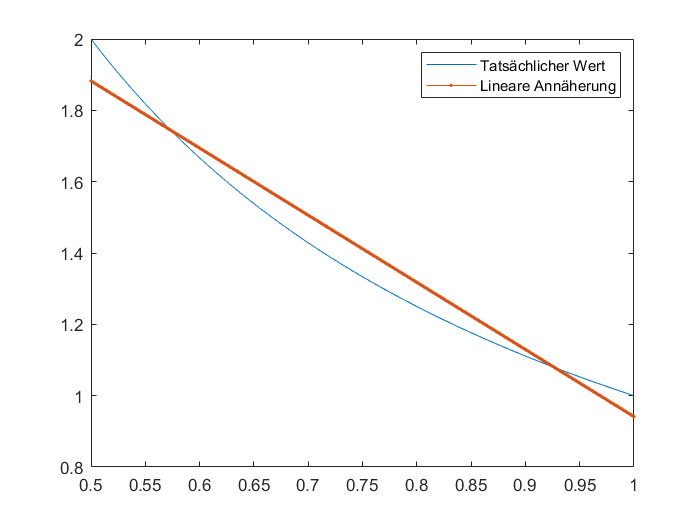
\includegraphics[width=0.7\textwidth]{Abbildungen/lineareApproximation.png}
		\caption{Graphische Darstellung der Annäherung}
	\end{figure}
	
	Der Fehler des Startwerts ist also maximal $\le \frac{1}{17}$. Da die Konvergenz der Newton-Raphson Division quadratisch ist, sich also der Fehler mit jeder Iteration quadriert reichen
	\begin{equation*}
		\lceil\log\textsubscript{2}\frac{n + 1}{\log\textsubscript{2}17}\rceil
	\end{equation*}
	Iterationsschritte um eine Genauigkeit von n Bit sicherzustellen.\cite{Vestias2013}
	
	\subsection{Genauigkeit der Formel zur Quadratwurzel auf n Bit}
	Für die Bestimmung der Genauigkeit wird das Produkt in der Approximation mit der Summenformel betrachtet. Für $i\ge1$ gilt:
	\begin{equation*}
		\prod_{k=1}^{i}\frac{2k - 1}{4k} = 
		\frac{2*1 - 1}{4 * 1}\prod_{k=2}^{i}\frac{2k - 1}{4k} =
		\frac{1}{4}\prod_{k=2}^{i}\frac{2k - 1}{4k}
	\end{equation*}
	Für den Term, der im Produkt sequentiell multipliziert wird gilt für $k \ge 1$: 
	\begin{equation*}
		\frac{2k - 1}{4k} < \frac{2k}{4k} = \frac{1}{2}
	\end{equation*}
	Daraus folgt:
	\begin{equation*}
		\frac{1}{4}\prod_{k=2}^{i}\frac{2k - 1}{4k} <
		\frac{1}{4}\prod_{k=2}^{i}\frac{1}{2}
	\end{equation*}
	\begin{equation*}
		\frac{1}{4}\prod_{k=2}^{i}\frac{1}{2} =
		\frac{1}{4}*2\textsuperscript{-i + 1} = 2\textsuperscript{-2} * 2\textsuperscript{-i + 1} = 2\textsuperscript{-i - 1}
	\end{equation*}
	Das entspricht einem k-Rechtsshift von $0,5$. Demnach hat die binäre Repräsentation das Ergebnis des Produkts stets mindestens i Nullen nach dem Komma.
	Für die Summe bedeutet das nun, dass die Summanden mit jeder Iteration eine Nachkommanull mehr haben als alle Vorherigen.
	
	Das heißt, dass $\sum_{i=1}^{n} \prod_{k=1}^{i} \frac{2k-1}{4k}$ alle Zahlen der Folge, die $\le$ n Nullen vor dem Komma haben aufaddiert. 
	
	Somit ist das Ergebnis auf n Bit genau.\newline
	
	Da hier aber der Wert der Summe mit Binary Splitting ermittelt wird und 
	\begin{equation*}
		\sum_{i=1}^{n} \prod_{k=1}^{i} \frac{2k-1}{4k} = 
		\frac{T(_{1,n + 1}) }{Q(_{1,n + 1}) }
	\end{equation*}
	gilt, muss für den Eingabewert zur Bestimmung des Zählers und Nenners $n + 1$ eingesetzt werden um n Bit Genauigkeit zu erhalten.
	
	\section{Performanzanalyse}
	Als Ansatz für eine Vergleichsimplementierung haben wir die Berechnung der Konstante durch die Summenformel der Einleitung gewählt. Zum Zeitpunkt der Abgabe ist die Implementierung der Formel nicht ausreichend genau um eine Referenz darstellen zu können.
	
	\subsection{Laufzeitverhalten des Programms}
	\begin{figure}[h]
		\centering
		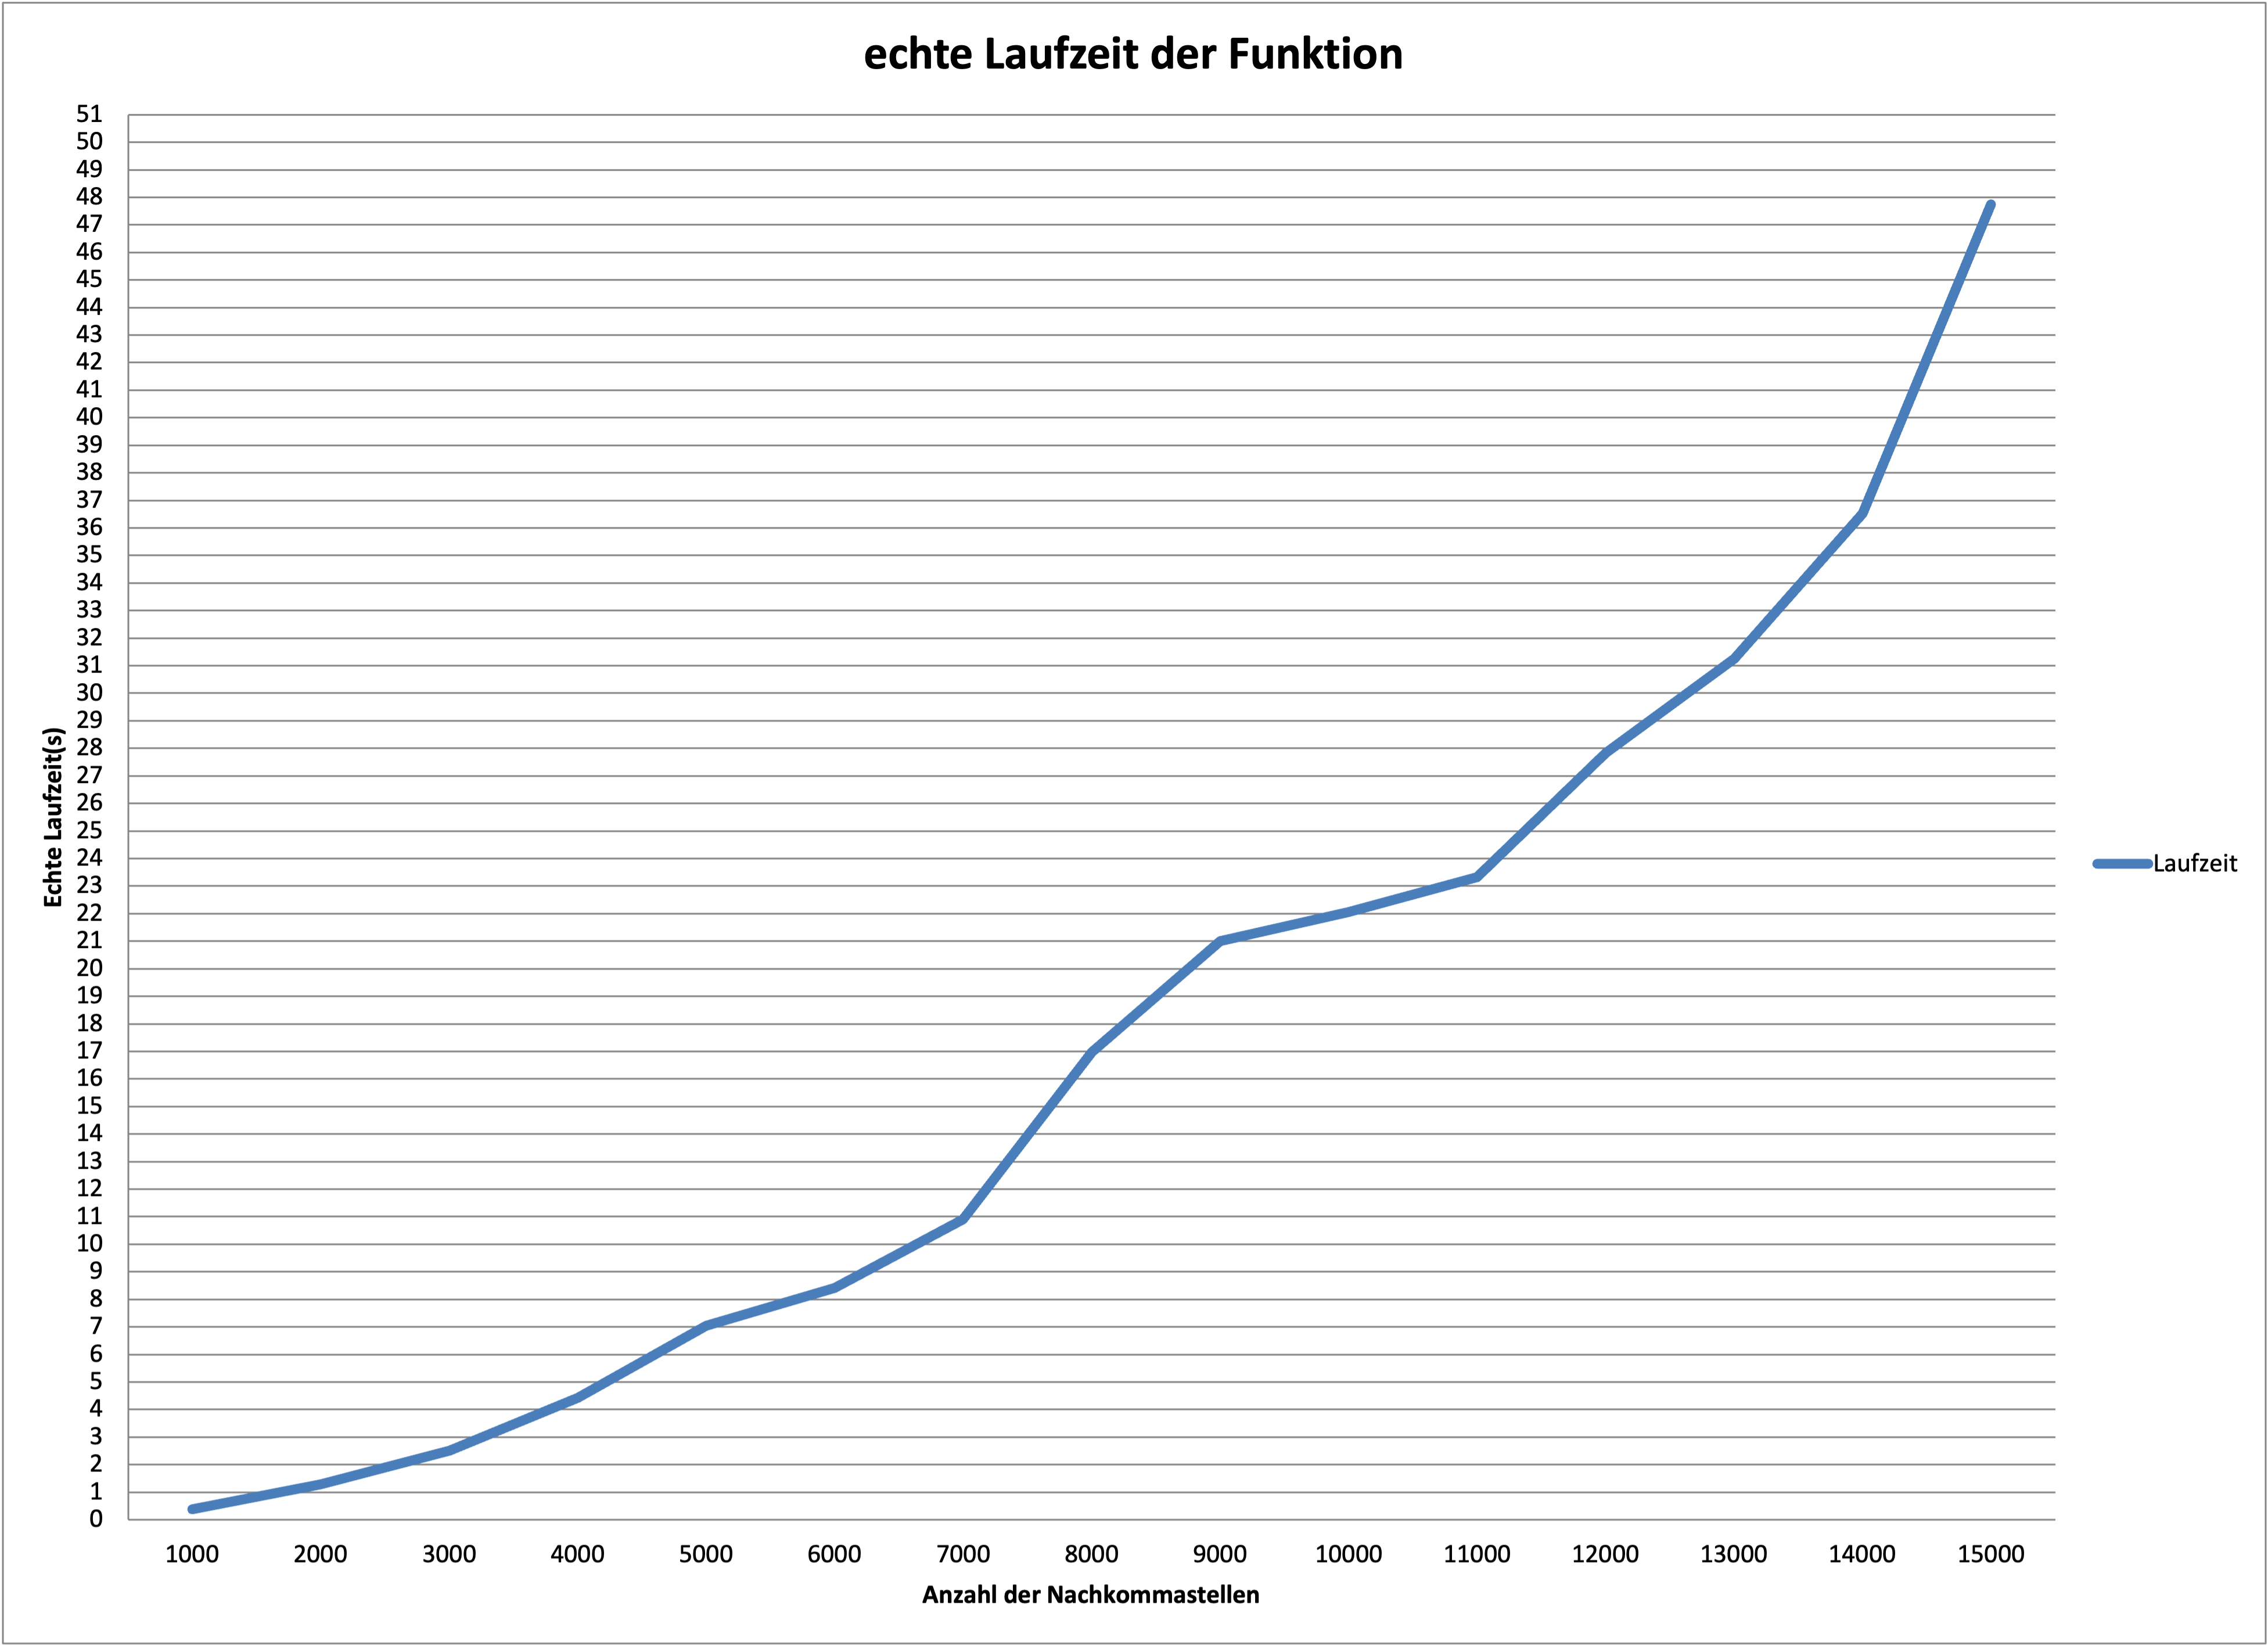
\includegraphics[width=0.8\textwidth]{Abbildungen/performanz.png}
		\caption{Durchschnittliche Laufzeit bei fünf Wiederholungen auf Intel i7-6700}
	\end{figure}
	
	Die Performanz nimmt bei größeren Eingabewerten stark zu. Dies wird vor allem von der Zunahme an Iterationen im Newton-Raphson Verfahren und der erhöhten Anzahl von Rekursionsschritten der Karazuba-Multiplikation verursacht. Ein möglicher Ansatz dies zu beheben ist, die Genauigkeit der Werte mit denen gerechnet wird zu beschränken. Dabei darf allerdings nicht die Genauigkeit des Resultats beeinträchtigt werden.
	
	\section{Zusammenfassung und Ausblick}
	\subsection{Zusammenfassung}
	Die Projektaufgabe besteht in der Approximation von $\sqrt{2}$. Dafür muss ein Konstrukt für große Zahlen und deren Arithmetik implementiert und anschließend genutzt werden, um die Konstante mittels Binary Splitting auf wählbare Genauigkeit anzunähern. 
	
	Das Konstrukt bignum speichert Zahlen als Aneinanderreihung von 32 Bit Blöcken in einem Feld mit einer Variable für die Länge des Feldes und der Nachkommablöcke. Es wird Karazuba-Multiplikation für das Bestimmen von Produkten und die Newton-Raphson Division für Quotienten benutzt. Beim Binary Splitting werden die Polynome so gewählt, dass das Ergebnis zu der in der Einleitung genannten Summenformel äquivalent ist.
	
	Durch ein Rahmenprogramm wird die Berechnung mit wählbaren Eingabefaktoren wie Genauigkeit und Zeitmessung dem Nutzer verfügbar gemacht.
	
	\subsection{Ausblick}
	Durch die Art wie die großen Zahlen gespeichert werden sind bedeutende Unkosten für die Speicherverwaltung nötig, wenn sich deren Anzahl an Blöcken ändert. Wenn man eine Abschätzung für die Größe der Zahlen findet, kann man die Anzahl der benötigten Speicherallozierungen durch Wiederverwendung bereits allozierter bignums deutlich verringern.
	
	% TODO: Fuegen Sie Ihre Quellen der Datei Ausarbeitung.bib hinzu
	% Referenzieren Sie diese dann mit \cite{}.
	% Beispiel: CR2 ist ein Register der x86-Architektur~\cite{intel2017man}.
	\bibliographystyle{plain}
	\bibliography{Ausarbeitung}{}
	
\end{document}
